\chapter{DDS \& RTPS}\label{Chapter:dds}
Data Distribution Service (DDS)\cite{DDS} e Real-Time Publish-Subscribe (RTPS)\cite{RTPS} sono strumenti che rivestono un ruolo importante nelle comunicazioni in sistemi distribuiti e \gls{Real-Time}. Infatti, anche se a diversi livelli, si occupano della la trasmissione di dati tra applicazioni e dispositivi interconnessi, giocando un ruolo importante in scenari con diverse centinaia di attori come i sistemi ad alte prestazioni come HPC. 


\section{Implementazione usasta}
In particolare, DDS e RTPS sono due differenti protocolli di comunicazione che accoppiati forniscono i servizi sopracitati . Ci sono state diverse implementazioni di questi protocolli da diversi società e organizzazioni, come:
\begin{itemize}
  \item FastDDS (eprosima)
  \item CycloneDDS (Oracle)
  \item ConnextDDS
  \item GurumDDS
\end{itemize}

In tutti i successivi capitoli verrà preso come riferimento FastDDS ed in particolare la sua versione 2.11.2 \cite{FastDDS}. E' stato scelto di utilizzare questa implementazione dato il supporto per le comunicazione Real-Time, e la vasta possibilità di impostazioni delle Qualità del servizio(QoS) che la rendevano adeguatamente configurabile per un utilizzo su sistemi di HPC. %TODO: Da migliorare

\section{DDS}
Data Distribution Service è un protocollo incentrato sullo scambio di dati per sistemi distribuiti. Questo si basa su modello chiamato Data-Centric Publish Subscribe (DCPS). I principali attori che vengono coinvolti sono:
\begin{itemize}
    \item Publisher: responsabile della creazione e configurazione dei DataWriter. Il DataWriter è l'entità responsabile della pubblicazione effettiva dei messaggi. Ciascuno avrà un Topic assegnato sotto il quale vengono pubblicati i messaggi;\label{actor:publisher}

    \item Subscriber: responsabile di ricevere i dati pubblicati sotto i topic ai quali si iscrive. Serve uno o più oggetti DataReader, che sono responsabili di comunicare la disponibilità di nuovi dati all'applicazione;\label{actor:subscriber}

    \item Topic: collega i DataWriter con i DataReader. È univoco all'interno di un dominio DDS;\@
    
    \item Dominio: utilizzato per collegare tutti i publisher e subscriber appartenenti a una o più domini di appartenenza, che scambiano dati sotto diversi topic. Il DomainParticipant funge da contenitore per altre entità DCPS, e svolge anche la funzione di costruttore di entità Publisher, Subscriber e Topic fornendo anche servizi di QoS;\@

    \item Partizione: costituisce un isolamento logico di entità all'interno dell'isolamento fisico offerto dal dominio;

\end{itemize}
Inoltre DDS definisce le cosiddette Qualità di Servizio (QoS policy) che servono configurare il comportamento di ognuno di questi attori.


\section{RTPS}
Real-Time Publisher Subscribe è un middleware\footnote{Formalmente è un protocollo a se stante, utilizzato da DDS come middleware} utilizzato da DDS per gestire la comunicazione su diversi protocolli di rete come UDP/TCP e Shared Memory. Il suo principale scopo è quello di inviare messaggi real-time, con un approccio best-effort e cercando di massimizzare l'efficienza. E' inoltre progettato per fornire strumenti per la comunicazione unicast e multicast. Le principali entità descritte da RTPS sono:
\begin{itemize}
    \item RTPSWriter: endpoint capace di inviare dati;
    \item RTPSReader: endpoint abilitato alla ricezione dei dati;
\end{itemize}
Ereditato da DDS anche RTPS ha la concezione di Dominio di comunicazione e come questo, le comunicazioni a livello di RTPS girano attorno al concetto di Topic prima definito. L'unità di comunicazione è chiamata \textbf{Change} che rappresenta appunto un cambiamento sui dati scritti sotto un certo topic. Ognuno degli attori registra questi \emph{Change} in una struttura dati che funge da cache.
In particolare la sequenza di scambio è:
\begin{enumerate}
    \item il \emph{change} viene aggiunto nella cache del RTPSWriter;
    \item RTPSWriter manda questa \emph{change} a tutti gli RTPSReader che conosce;
    \item quando RTPSReader riceve il messaggio, aggiorna la sua cache con il nuovo \emph{change}.
\end{enumerate}

\begin{figure}[H]
    \centering
    \begin{subfigure}{0.45\linewidth}
      \centering
      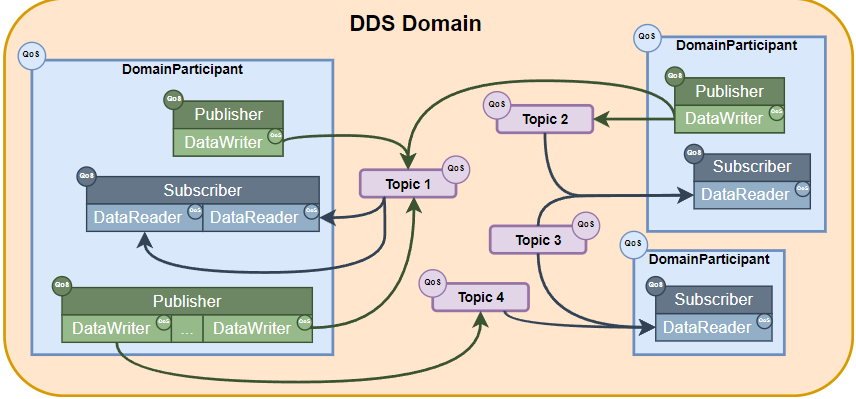
\includegraphics[width=\linewidth]{./img/dds_architecture.png}
      \caption{Schema DDS}\label{fig:dds}
    \end{subfigure}
    \begin{subfigure}{0.45\linewidth}
      \centering
      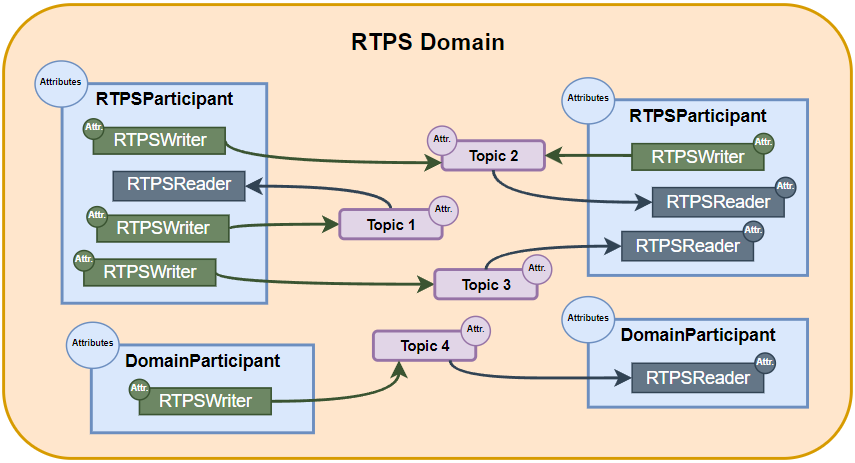
\includegraphics[width=\linewidth]{./img/rtps_architecture.png}
      \caption{Schema RTPS}\label{fig:rtps}
    \end{subfigure}
    \caption{Confronto tra architettura DDS e RTPS}\label{fig:confrontodds_rtps}
  \end{figure}

%TODO: ROS

\section{ROS}\label{SSEC:rosiface}


Questo approccio distribuito per lo scambio dei dati tra vari attori utilizzando un middlware basato su DDS non è idea inedita. Infatti dalla sua seconda versione il software open-source \textbf{Robot Operating System}\cite{ros2iron} meglio conosciuto come ROS
\begin{wrapfigure}{r}{0.5\textwidth}
  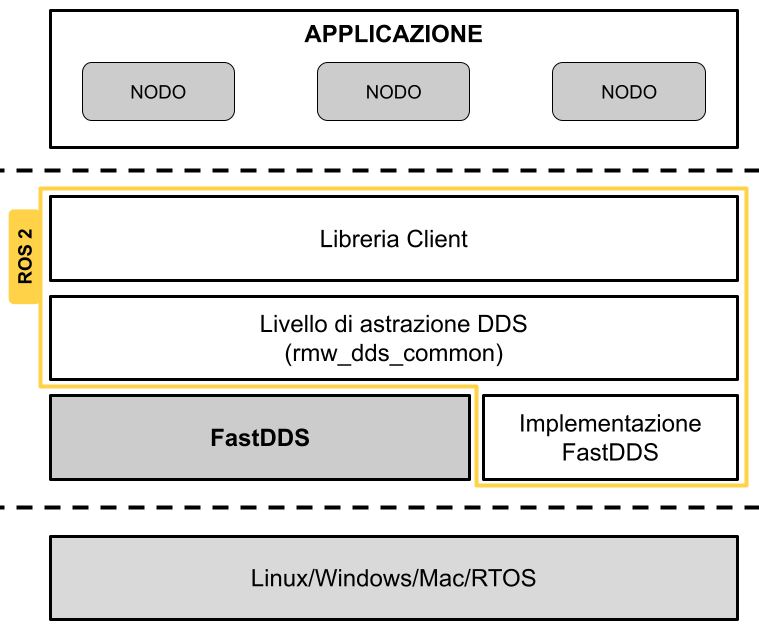
\includegraphics[width=0.5\textwidth]{img/ROS_MW.png}
  \caption{Ros Middleware per DDS} 
  \label{fig:rmw_dds_common}
\end{wrapfigure}
ha deciso di usare questi strumenti introducendo un ulteriore livello che permette di usare diverse implementazioni di DDS. Questa idea è stata e sarà di grande ispirazione per il completamento di questo progetto.
Nello specifico, è stata creata una libreria chiama rmw\_dds\_common(ros middleware) come mostrato nella \ref{fig:rmw_dds_common}\footnote{L'implementazione di FastDDS vuole essere un esempio tra le diverse soluzioni disponibili per ROS2} sopra il quale la community ha creato le implementazioni di DDS desiderate, andando a creare così diverse possibilità di configurazione dello stesso servizio di distribuzione dati.
Inoltre per cambiare tra le diverse versioni di DDS si deve semplicemente impostare una variabile di ambiente, rendendo il procedimento facile per tutti i possibili fruitori di ROS2. 

Tuttavia è stato scelto di utilizzare direttamente l'implementazione DDS invece che \emph{Ros middlware} per i seguenti motivi:
\begin{itemize}
    \item Potenzialità: ROS mette a disposizione solo alcuni degli strumenti resi disponibili dallo strato DDS, andando a limitare la possibilità di sfruttamento di tutte le impostazioni e QoS di FastDDS;
    \item Granularità: oltre alla mancanza di alcune funzionalità, in ros sono predisposti dei pacchetti preconfigurati di entità. Per andare a studiare più approfonditamente gli strumenti su architetture diverse, è più pratico avere la possibilità di cambiare ogni piccola configurazione.
    \item Flessibilità: Per andare a definire delle strutture dati di ROS, al fine di scambiare messaggi DDS usando il middleware offerto, era necessario creare diverse strutture dati che combaciassero con le interfacce ROS;
    \item Diversa natura: In ROS, la maggior parte delle comunicazioni fatte sono intra-processo e raramente viene utilizzata una infrastruttura di rete, per andare a collegare tutti i nodi. Per questo sono maggiormente ottimizzate quel tipo di comunicazioni, piuttosto che quelle su rete, come in questo caso.
    \item Facilità di implementazione: Implementare completamente \emph{rmw\_dds\_common} richiedeva un impegno e uno studio non indifferente della architettura sottostante a ROS, che seppur ben documentata, sarebbe costata diverso tempo. 
\end{itemize}


% in ROS, la maggior parte delle comunicazioni fatte sono intra-processo e raramente viene utilizzata una infrastruttura di rete, per andare a scambiare dei messaggi. Per questo sono maggiormente ottimizzate quel tipo di comunicazioni, piuttosto che quelle su rete, come nel caso di HPC


% Ros Middleware interface\cite{ros2iface}, developed within the context of the Robot Operating System (ROS), stands as a pinnacle of innovation in the realm of creating middleware for Distributed Data Systems. The middleware leverages advanced data serialization techniques, optimized for real-time performance and efficient data exchange. Its incorporation of Quality of Service parameters and support for both publish-subscribe and request-response communication patterns underscores its sophistication, making it a state-of-the-art choice for building DDS middleware in distributed environments.

% In fact ROS capitalizes on the Data Distribution Service as a foundational communication middleware protocol\cite{ros2iron}, which plays a pivotal role in enabling seamless and efficient data exchange and interaction between the myriad components that constitute a robotic ecosystem.

% The structure of the middleware-ROS, exemplified by \emph{rmw\_dds\_common}\cite{ros2iron}, combined with various middleware specific to each DDS service provider, also allows for easy switching of the DDS implementation using a simple variable change, invoked before launching the ROS-node, among the many available options (FastDDS, CycloneDDS, ConnextDDS, etc.). 
% This approach permits choosing the most suitable DDS implementation for specific use case. For instance, if we intend to use FastDDS (most suitable one for real-time communications) as the primary DDS service, we can set \emph{rmw\_implementation=fastdds}, and ROS will be able to abstract all of its functions.